\subsection{Subclasses}

\nbgpara{1}{} Before we state the first axioms, it is necessary to establish one more piece of descriptive language. Membership (\(\in\)) describes a relation between a class and a potential element. But as we articulate the rules of set theory, we will frequently need to compare classes to other classes. Once membership has been introduced, we can build a second, broader relation: the relation of one entire class being contained in another. Unlike membership, this relation is not primitive; it is defined entirely in terms of \(\in\).

\begin{definition}[Subclass]\label{def:subclass}
Let \(A\) and \(B\) be classes.

We write that \(A \subseteq B\) (i.e., that \(A\) is a \textit{subclass} of \(B\), or that \(A\) is \textit{contained in} \(B\)), iff every element of \(A\) is also an element of \(B\).

In symbols:
$$
A \subseteq B \quad \defequiv \quad \forall x\,(x \in A \to x \in B).
$$
\end{definition}

\nbgpara{2}{} For example, if \(A = \{a,b\}\) and \(B = \{a,b,c\},\) then \(A \subseteq B\), since every element of \(A\) is also an element of \(B\). The class \(B\) contains everything that \(A\) contains, and possibly more. On a first pass, the metaphor of \sideLink{subclass}{spatial containment} helpfully visualizes this relationship.

\begin{sideillustration}[subclass]
\begin{figure}[h]
\centering
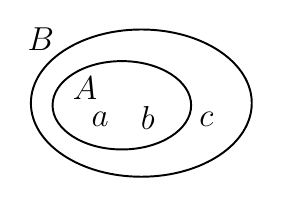
\begin{tikzpicture}[x=0.55cm,y=0.55cm,every node/.style={inner sep=0pt}]

    % The class B
    \draw[line width=0.7pt] (0,0) ellipse (2.55 and 1.70);
    \node[font=\large] at (-2.32,1.48) {$B$};

    % The class A inside B
    \draw[line width=0.7pt] (-0.45,-0.05) ellipse (1.6 and 1.02);
    \node[font=\large] at (-1.30,0.35) {$A$};

    % Members
    \node[font=\large] at (-0.95,-0.38) {$a$};
    \node[font=\large] at (0.15,-0.34) {$b$};
    \node[font=\large] at (1.5,-0.38) {$c$};

\end{tikzpicture}
\caption{If \(A=\{a,b\}\) and \(B=\{a,b,c\}\), then \(A \subseteq B\).}
\end{figure}
\end{sideillustration}

\nbgpara{3}{} \quad By contrast, if \(C = \{c,d\}\), then \(C \nsubseteq B\), since \(d \in C\), but \(d \notin B\). To show that one class is not a subclass of another, it is enough to find a single element of the first class that is missing from the second. Again, the metaphor of \sideLink{subclass2}{spatial containment} provides a helpful visualization.

\begin{sideillustration}[subclass2]
\begin{figure}[h]
\centering
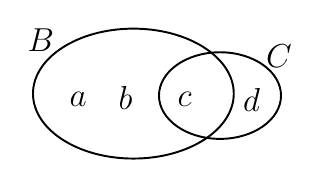
\begin{tikzpicture}[x=0.5cm,y=0.5cm,every node/.style={inner sep=0pt}]

    % The class B
    \draw[line width=0.7pt] (-0.75,0) ellipse (2.55 and 1.65);
    \node[font=\large] at (-3.10,1.35) {$B$};

    % The class C
    \draw[line width=0.7pt] (1.45,-0.05) ellipse (1.55 and 1.10);
    \node[font=\large] at (2.95,0.95) {$C$};

    % Members of B but not C
    \node[font=\large] at (-2.15,-0.15) {$a$};
    \node[font=\large] at (-0.95,-0.11) {$b$};

    % Member of both B and C
    \node[font=\large] at (0.55,-0.15) {$c$};

    % Member of C but not B
    \node[font=\large] at (2.25,-0.15) {$d$};

\end{tikzpicture}
\caption{If \(C=\{c,d\}\) and \(B=\{a,b,c\}\), then \(C \nsubseteq B\).}
\end{figure}
\end{sideillustration}

\nbgpara{4}{} Notice that the statement \(A \subseteq B\) does not say that \(A\) is itself an element of \(B\). It says that every element of \(A\) is an element of \(B\). Thus, \(A \subseteq B\) and \(A \in B\) are profoundly different statements. The first compares two classes by checking their contents against each other; the second treats \(A\) as a single entity and states that this entity is one of the members collected inside \(B\).

\nbgpara{5}{} The preceding diagrams may make it tempting to think of subclasshood as a relation in which one class is visibly smaller than another. This is a useful picture in many cases, but it is not part of the definition. In particular, Definition~\ref{def:subclass} implies that every class is a subclass of itself. 

\begin{proposition}[Subclasshood Is Reflexive]\label{prop:subclasshood-reflexive}
\[
\forall x(x\subseteq x).
\]
\end{proposition}

\begin{proof}
Let \(A\) be an arbitrary class. To show that \(A \subseteq A\), we must show that every element of \(A\) is also an element of \(A\). But this is immediate: if \(x \in A\), then \(x \in A\). Hence \(A \subseteq A\). Since $A$ was arbitrary, Proposition \ref{prop:subclasshood-reflexive} follows by Universal Generalization.
\end{proof}

If we tried to draw this case, the two boundaries would simply coincide; there is therefore no very helpful picture to add. Note that the quantifier in Proposition \ref{prop:subclasshood-reflexive} is entirely unrestricted: It ranges over the \textit{entire} domain of set theory, i.e., all classes whatsoever. 

\nbgpara{6}{} This is why subclasshood should not be understood as meaning ``properly smaller than." A class may be contained in another class even when the two classes are identical. Loosely put, a relation is \textit{reflexive} iff every object stands in that relation to itself. We will make the concept of a relation, and properties such as reflexivity, more precise later. For now, the intuitive idea is enough. Identity is another familiar example of a reflexive relation: for every object \(x\), we have \(x = x\).

\nbgpara{7}{} So, if we want to say that one class is contained in another, but is not identical to it, we need a stricter notion. This leads to the definition of a \textit{proper subclass}.

\begin{definition}[Proper Subclass]\label{def:proper-subclass}
Let \(A\) and \(B\) be classes.

We write that \(A \subset B\) (i.e., that \(A\) is a \textit{proper subclass} of \(B\)), iff \(A \subseteq B\) and \(A \neq B\).

In symbols:
\[A \subset B \quad \defequiv \quad A \subseteq B \ \land \ A \neq B\]
\end{definition}

\nbgpara{8}{} \quad Consider \(A = \{a,b\}\) and \(B = \{a,b,c\}\) once more. We have already seen that \(A \subseteq B\). But \(A\) and \(B\) are not identical, since \(c \in B\) while \(c \notin A\). Thus, \(A\) is not merely a subclass of \(B\), but a proper subclass of \(B\). This is visually obvious in Figure 2.

\nbgpara{9}{} \quad By contrast, \(A \subseteq A\), but it is not the case that \(A \subset A\). A class cannot be a proper subclass of itself, because proper subclasshood requires inequality. 

\begin{proposition}[Proper Subclasshood is Anti-Reflexive]
    \[\forall x(x \not\subset x)\]
\end{proposition}

\begin{proof}
    Let $A$ be an arbitrary class. By the reflexivity of identity, we have $A=A$, i.e., it is not the case that $A \neq A$. Thus, the second conjunct of Definition \ref{def:proper-subclass} is not fulfilled, and hence $A \not\subset A$.
\end{proof}

Thus, \(\subseteq\) allows equality, while \(\subset\) excludes it. The visual similarity to the symbols for numerical inequality is intentional: in terms of allowing or forbidding equality, \(\subseteq\) resembles \(\leq\), and \(\subset\) resembles \(<\).

\nbgpara{10}{} However, this analogy with numbers carries a hidden danger, and we must be careful about which intuitions we draw from it. For any two numbers \(n\) and \(m\), they can always be compared: either \(n \leq m\) or \(m \leq n\). Numbers lie on a single, ordered line. Classes, by contrast, generally do not. If \(A = \{a,b\}\) and \(B = \{b,c\}\), neither class is contained in the other. Even though they share an element, \(A \nsubseteq B\) (because \(a \notin B\)) and \(B \nsubseteq A\) (because \(c \notin A\)). Thus, it is perfectly possible for both to be true simultaneously. Subclasshood tells us how classes are nested, but it does not force all classes into a single linear order.

\nbgpara{11}{} We shall use \(\subseteq\) for subclasshood in general, allowing equality, and \(\subset\) for proper subclasshood, excluding equality. Be aware that some authors use these symbols differently. It is common in other literature to see \(\subset\) used for general subclasses (what we write as \(\subseteq\)), and \(\subsetneq\) used for proper subclasses. However, our convention will be fixed throughout this text.

\nbgpara{12}{} Finally, the phrase \textit{proper subclass} should not be confused with the phrase \textit{proper class}. A proper subclass is a class strictly contained in another class. A proper class, by contrast, will mean a class that is too large to be a set.